\documentclass{beamer}

% Setup appearance:

%\usetheme{Darmstadt}
%\usetheme{Warsaw}
%\usetheme{Boadilla}
%\usetheme{Hannover}   %jó
%\usetheme{Marburg}      %jó
%\usetheme{Singapore}  %jó
%\usetheme{Szeged}
\usetheme{CambridgeUS}

%color theme
\usecolortheme{beaver}
%\usecolortheme{reen}


\usepackage[magyar]{babel}
%\usepackage[english]{babel}

\usepackage[utf8]{inputenc}
\usepackage{times}
\usepackage[T1]{fontenc}

\usepackage{amsmath}
\usepackage{graphicx}
\usepackage{enumerate}

\usepackage{caption}
%\usepackage{subcaption}

\usepackage{epstopdf}

\usepackage{color}
\usepackage{listings}
\definecolor{javared}{rgb}{0.6,0,0} % for strings
\definecolor{javagreen}{rgb}{0.25,0.5,0.35} % comments
\definecolor{javapurple}{rgb}{0.5,0,0.35} % keywords
\definecolor{javadocblue}{rgb}{0.25,0.35,0.75} % javadoc
 
\definecolor{dkgreen}{rgb}{0,.6,0}
\definecolor{dkblue}{rgb}{0,0,.6}
\definecolor{dkyellow}{cmyk}{0,0,.8,.3}

\lstset{
  language        = php,
  basicstyle      = \small\ttfamily,
  keywordstyle    = \color{dkblue},
  stringstyle     = \color{red},
  identifierstyle = \color{dkgreen},
  commentstyle    = \color{gray},
  emph            =[1]{php},
  emphstyle       =[1]\color{black},
  emph            =[2]{if,and,or,else},
  emphstyle       =[2]\color{dkyellow}}
 
%\lstset{language=Java,
%basicstyle=\ttfamily,
%keywordstyle=\color{javapurple}\bfseries,
%stringstyle=\color{javared},
%commentstyle=\color{javagreen},
%morecomment=[s][\color{javadocblue}]{/**}{*/},
%numbers=left,
%numberstyle=\tiny\color{black},
%stepnumber=2,
%numbersep=10pt,
%tabsize=4,
%showspaces=false,
%showstringspaces=false}
%\lstset{
%language=HTML,
%basicstyle=\ttfamily,
%keywordstyle=\color{blue},
%breaklines=true, 
%commentstyle=\color{javagreen},
%numbers=left,
%numberstyle=\tiny\color{gray},
%stepnumber=2,
%numbersep=5pt,
%}


\definecolor{okgreen}{rgb}{0,1,0}
\definecolor{wrongred}{rgb}{1,0,0}

\newcommand{\OK}{{\color{okgreen}\checkmark}}
\newcommand{\WRONG}{{\color{wrongred}X}}
\newcommand{\QUESTION}[1]{{\color{wrongred}¿} #1 {\color{wrongred}?}}
\newcommand{\QUESTIONMARK}{{\color{wrongred}?}}
\newcommand*{\supervisor}[1]{\def\supname{#1}}

% Author, Title, etc.

\title[Android Fejlesztés]{Szoftverfejlesztés Android platformra}

\author{Adam Satan}

\institute{Minőségbiztosítás informatikája}

\date{\the\year}

\begin{document}

\maketitle
%\begin{frame}
%  \titlepage
%\end{frame}

\section{Bevezető}

\begin{frame}[fragile]{Android}
	\begin{minipage}{0.49\textwidth}		
		\begin{itemize}
			\item Google - Android
			\item Android Studio
			\item Fejleszési nyelvek
			\item Szoftver fejlesztés
			\item Szoftver tesztelés	
		\end{itemize}
	\end{minipage}
	\begin{minipage}{0.49\textwidth}
		
\includegraphics[width=1 \linewidth]{figures/android.png}
	\end{minipage}
\end{frame}
\begin{frame}[fragile]{Google LCC}
	\begin{minipage}{0.49\textwidth}
		\begin{itemize}
				\item 19 éve alapították
				\item Fő bevételforrása: reklámok
				\item kb 73000 alkalmazott
				\item 767 Milliárd dolláros piaci érték
				\item Magyarország GDP-je: 120 Milliárd dollár 
		\end{itemize}
	\end{minipage}
\begin{minipage}{0.49\textwidth}
	\begin{itemize}
		\item Ismertebb munkásságai:
		\begin{itemize}
			\item Google kereső
			\item Gmail
			\item Chrome
			\item Fiber
			\item Maps
			\item Docs, Drive
			\item Chromebook
			\item Android
		\end{itemize}
	\end{itemize}
\end{minipage}
\end{frame}
\begin{frame}[fragile]{Google}
	\begin{minipage}{0.8\textwidth}
		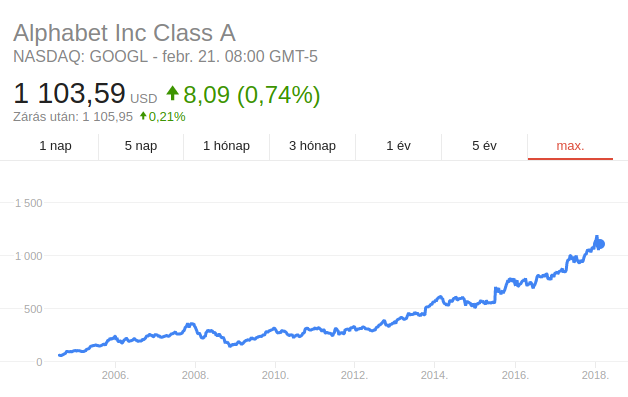
\includegraphics[width=1 \linewidth]{figures/share.png}
	\end{minipage}
\end{frame}
\begin{frame}[fragile]{Android}
	\begin{minipage}{0.49\textwidth}
		\begin{itemize}
			\item 2008 szeptember
			\item Linux alapú mobil operációs rendszer
			\item ARM, x86, x64
			\item Telefon, Tablet, Okosóra, TV, Autó
		\end{itemize}
	\end{minipage}
	\begin{minipage}{.49\textwidth}
		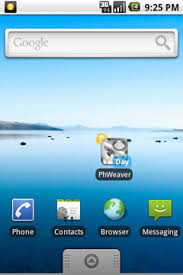
\includegraphics[width=.8\linewidth]{figures/android10.jpeg}
	\end{minipage}
\end{frame}
\begin{frame}[fragile]{Android}
	\begin{minipage}{0.49\textwidth}
		\begin{itemize}
			\item 8. verzió (2017 December)
			\item 432 millió okos telefonból 352 millió androidos (87\%)
			\item 3,638,448 alkalmazás (2018 febr. 20)
			\item Átlagosan havonta 60,000 új app
		\end{itemize}
	\end{minipage}
	\begin{minipage}{.49\textwidth}
		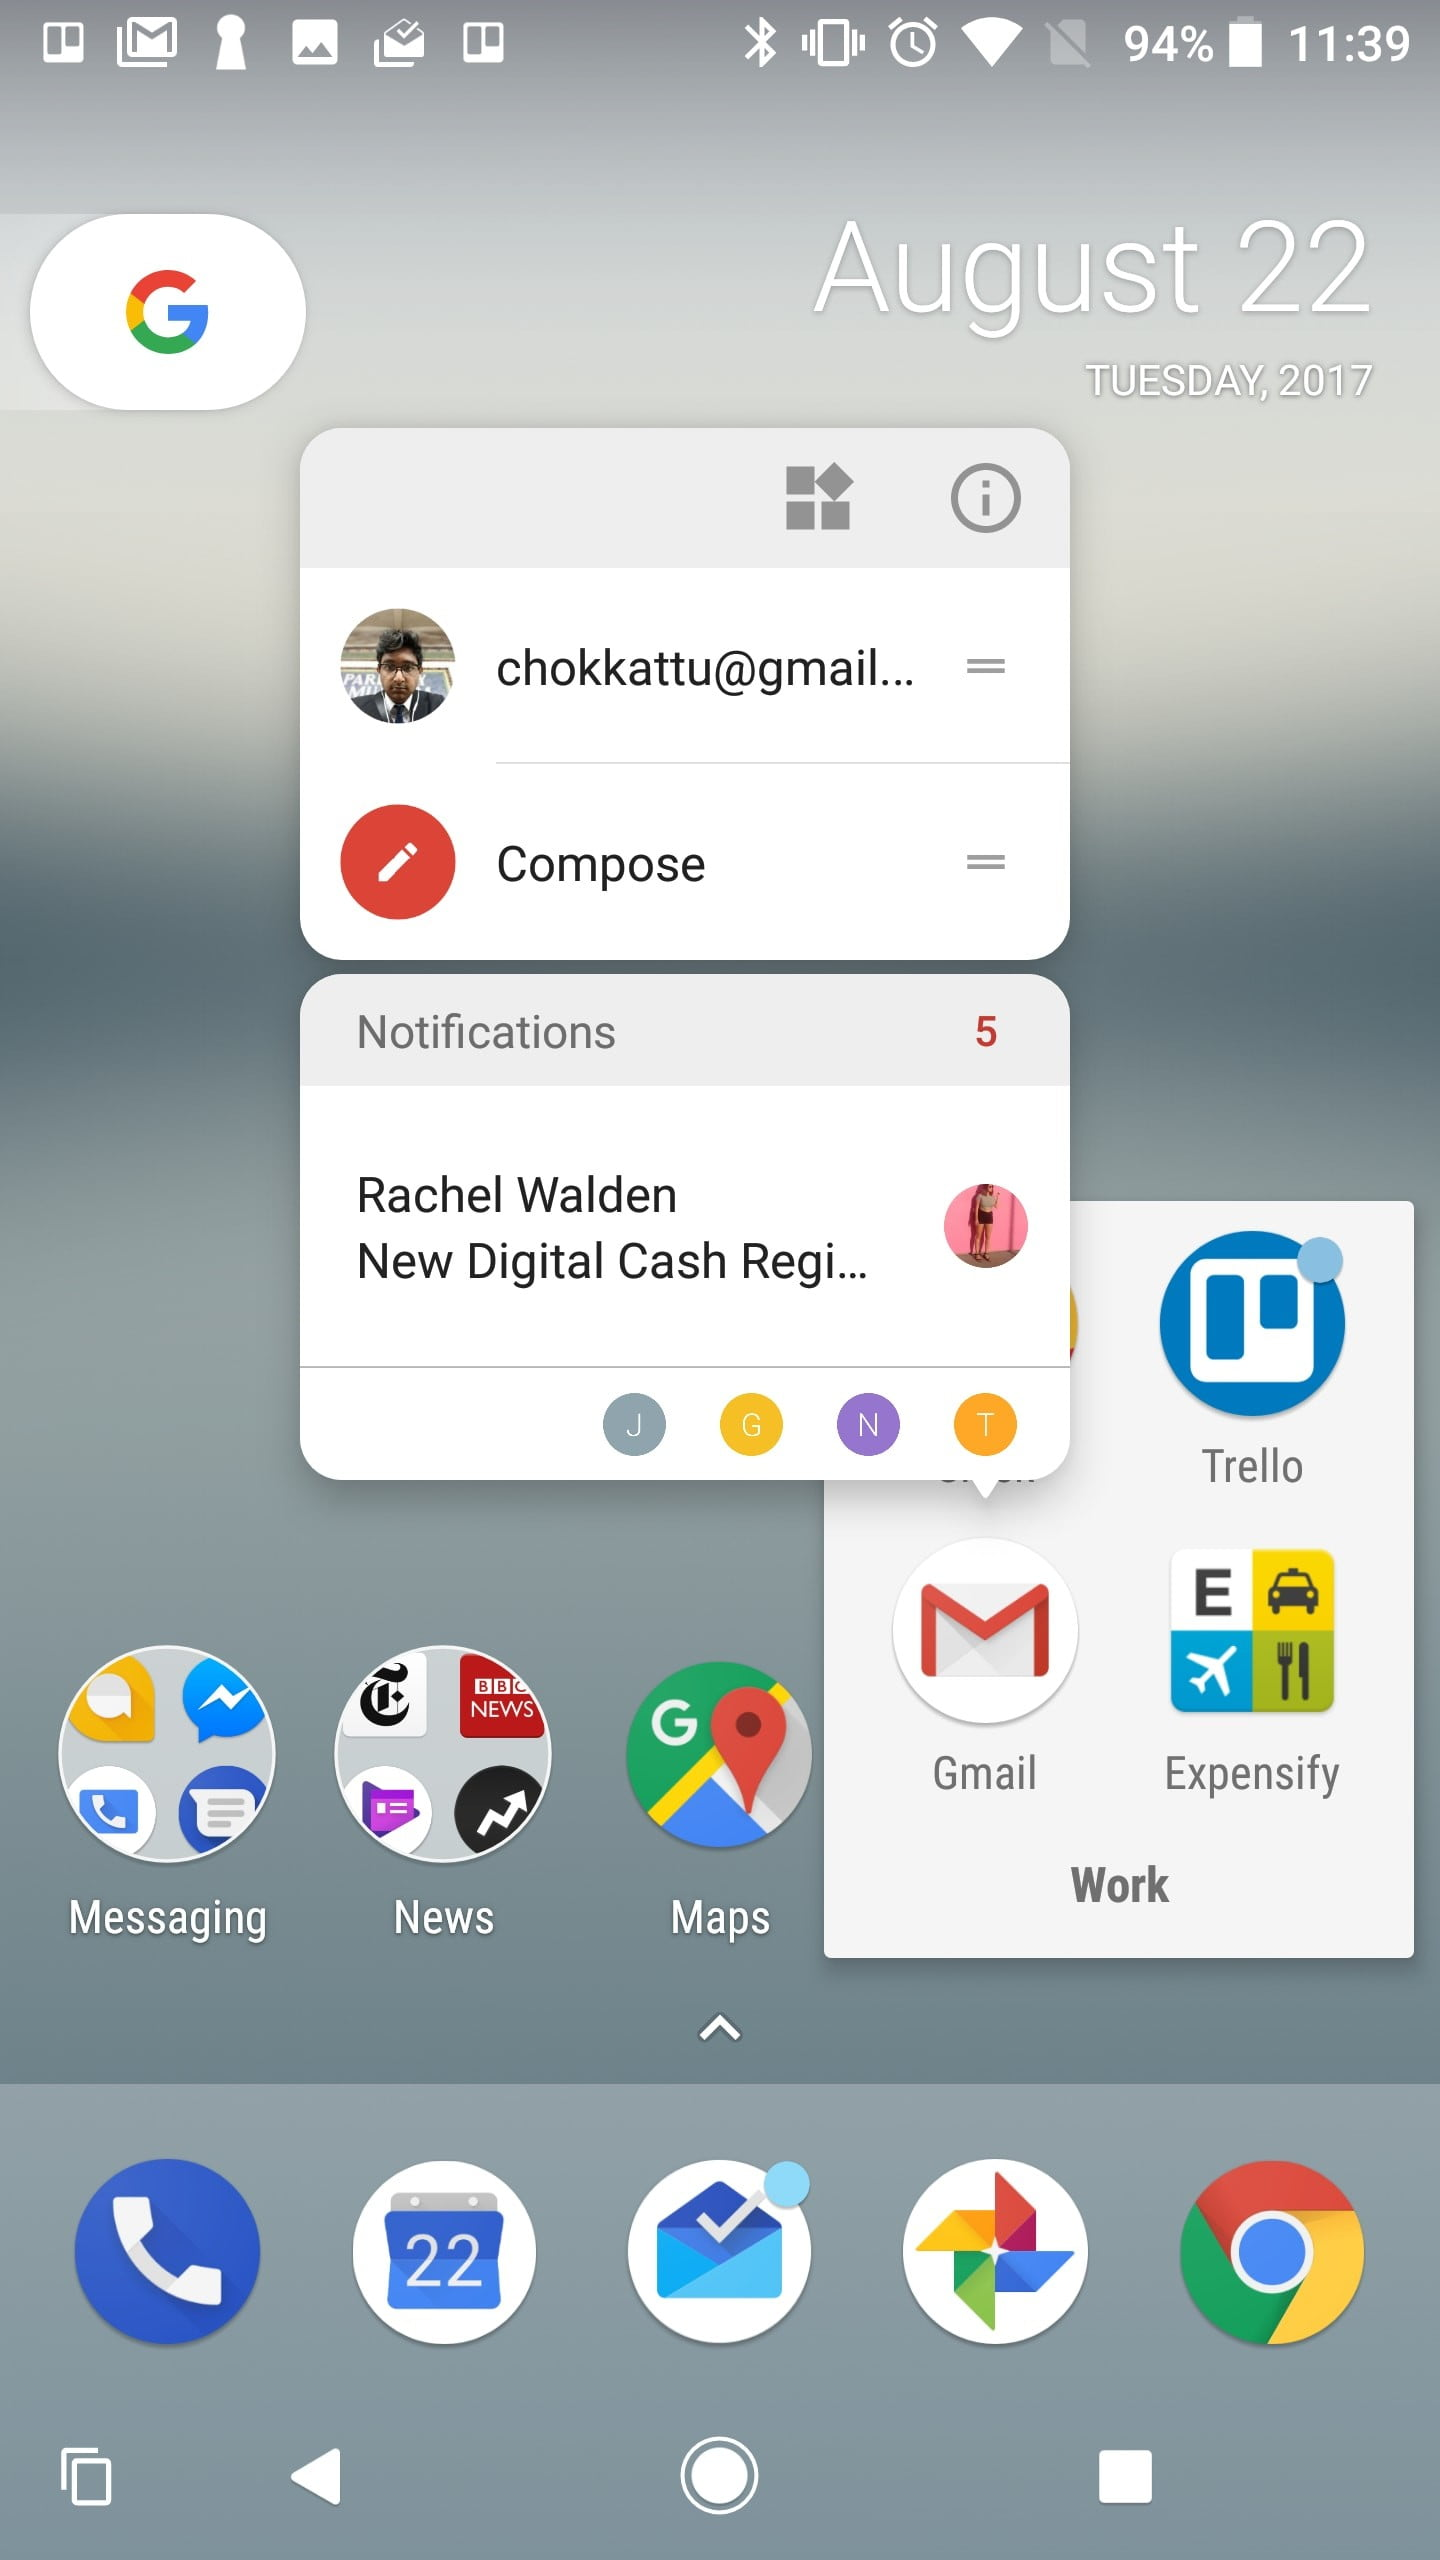
\includegraphics[width=.8\linewidth]{figures/android80.jpg}
	\end{minipage}
\end{frame}
\begin{frame}[fragile]{Android fejlesztő}
	\begin{minipage}{0.49\textwidth}
		\begin{itemize}
			\item 80000\$ átlagfizetés (70000\$ átlag fejlesztői fizetés)
			\item 1,000,000 reklámos alkalmazás
			\item 3.5 milliárd \$ reklámkifizetés 2012 óta
		\end{itemize}
	\end{minipage}
	\begin{minipage}{.49\textwidth}
		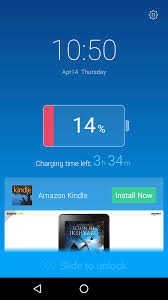
\includegraphics[width=.8\linewidth]{figures/androidad.jpeg}
	\end{minipage}
\end{frame}
\section{Fejlesztési nyelvek}
\begin{frame}[fragile]{Kotlin}
	\begin{minipage}{0.45\textwidth}
		\begin{itemize}
			\item Erősen típusos programozási nyelv
			\item Orosz fejlesztésű
			\item IDEA/Android Studio fejlesztői készítették
			\item Lásd következő előadást
		\end{itemize}
	\end{minipage}
	\begin{minipage}{0.49\textwidth}
		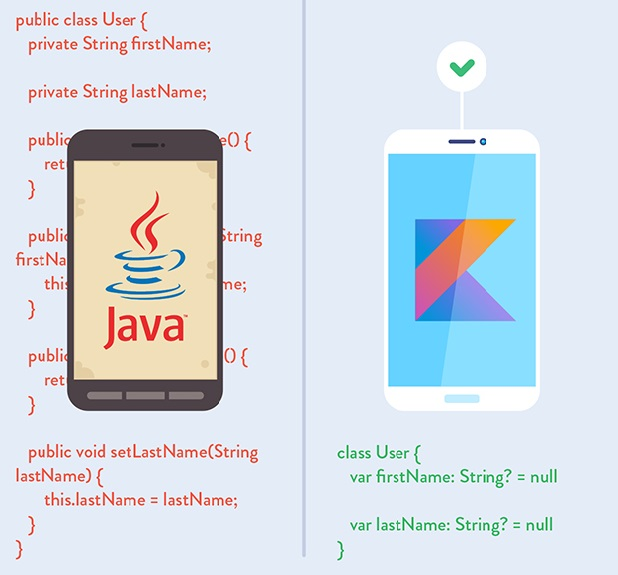
\includegraphics[width=1\linewidth]{figures/Kotlin-Vs-Java.jpg}
	\end{minipage}
\end{frame}
\begin{frame}[fragile]{Java}
	\begin{minipage}{0.9\textwidth}
		\begin{itemize}
			\item Objektum orientált nyelv
			\item Az Android hivatalos nyelve
			\item Extrák
			\begin{itemize}
				\item region kezelés
				\item Callback metódusok
			\end{itemize}
			\item APK-ra csomagolódik
		\end{itemize}
	\end{minipage}
	\begin{minipage}{1\textheight}
		\centering
		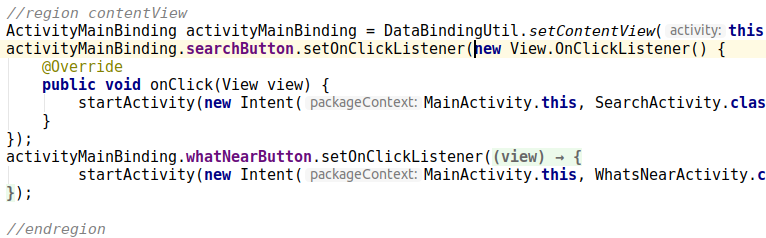
\includegraphics[width=1\linewidth]{figures/regionCallback.jpg}
	\end{minipage}
\end{frame}
\begin{frame}[fragile]{XML}
	\begin{minipage}{0.40\textwidth}
		\begin{itemize}
			\item AndroidManifest.xml
			\item GUI elrendezés leírása
			\item Nyelviesítési fájlok
			\item Vektorgrafikus képek
		\end{itemize}
	\end{minipage}
\begin{minipage}{.59\textheight}
	\centering
	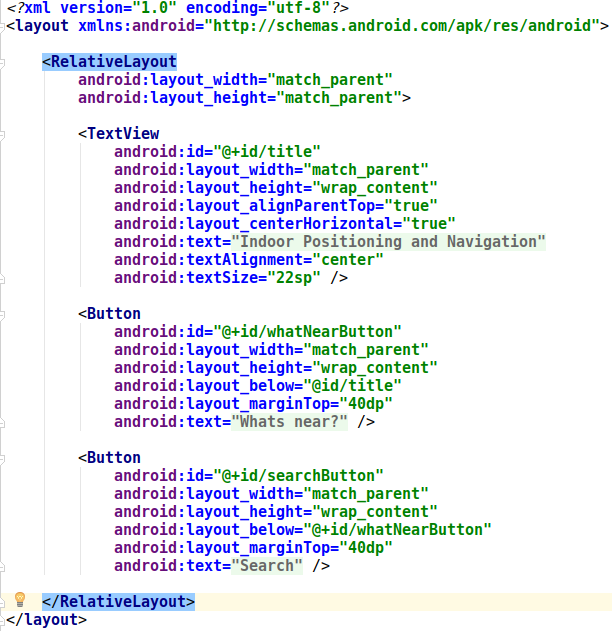
\includegraphics[width=1\linewidth]{figures/layout.png}
\end{minipage}
\end{frame}
\begin{frame}[fragile]{C\# - Mono}
	\begin{minipage}{0.49\textwidth}
		\begin{itemize}
			\item Xamarin kiegészítő kell hozzá
			\item Képes majdnem minden platformra fejleszteni(iOS, Android, Windows, Mac)
			\item GUI irányelvek ütköznek
		\end{itemize}
	\end{minipage}
	\begin{minipage}{.69\textheight}
		\centering
		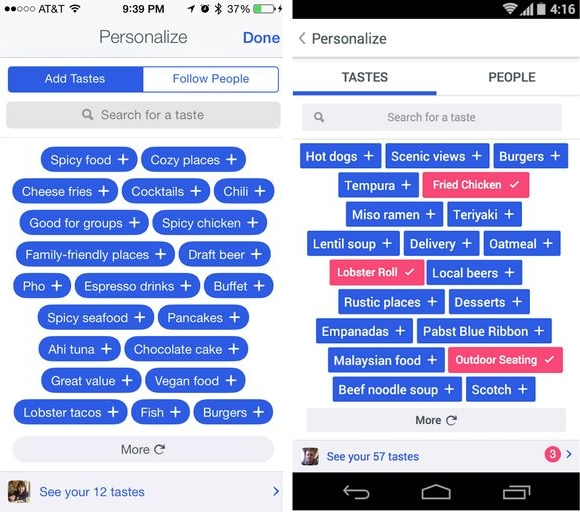
\includegraphics[width=1\linewidth]{figures/iosvsandroid.jpg}
	\end{minipage}
\end{frame}
\section{Androidra fejlesztés}
\begin{frame}[fragile]{Android Studio}
	\begin{minipage}{0.45\textwidth}
		\begin{itemize}
			\item IntelliJ IDEA-ra épül
			\item Hivatalos Android fejlesztőkörnyezet
			\item Elérhető minden platformra
		\end{itemize}
	\end{minipage}
	\begin{minipage}{0.45\textwidth}
		
\includegraphics[width=1\linewidth]{figures/ass.png}
	\end{minipage}
\end{frame}
\begin{frame}[fragile]{Android Studio}
	\begin{minipage}{0.9\textwidth}
		\begin{itemize}
			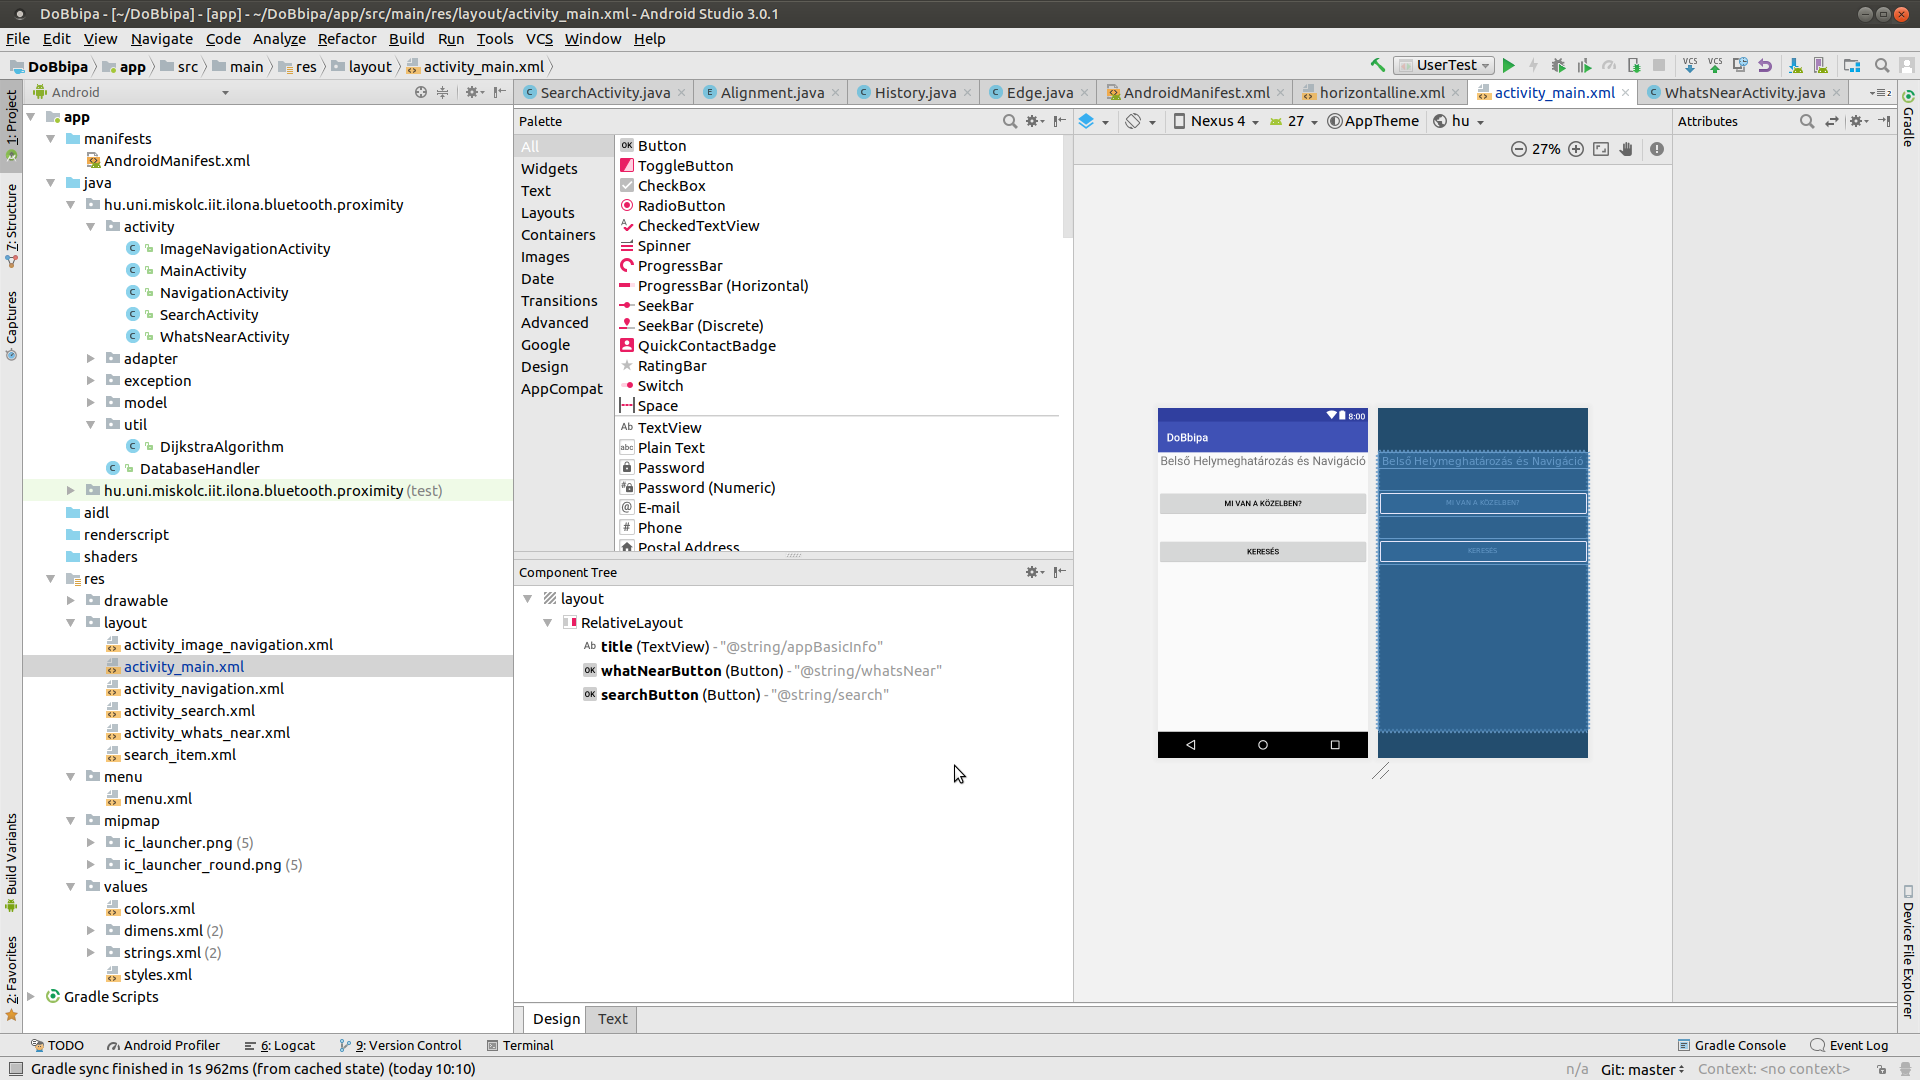
\includegraphics[width=1\linewidth]{figures/androidStudio.png}
		\end{itemize}
	\end{minipage}
\end{frame}
\begin{frame}[fragile]{Verzió választás}
	\begin{minipage}{0.29\textwidth}
		\begin{itemize}
			\item Különböző Android verziókhoz különböző API szintek
			\item pl Android 6.0 = API 23
		\end{itemize}
	\end{minipage}
	\begin{minipage}{0.70\textwidth}
		\begin{itemize}
			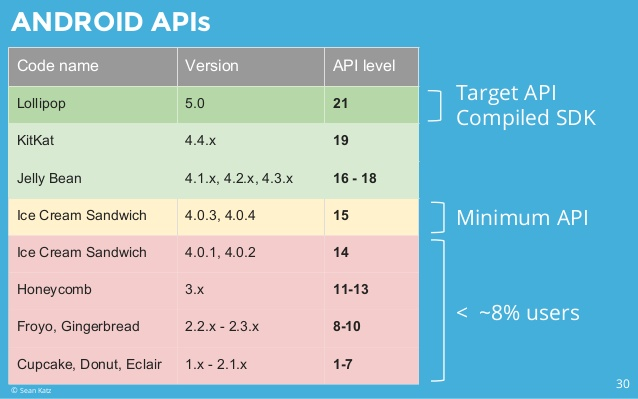
\includegraphics[width=1\linewidth]{figures/android-best-practices-2015-30-638.jpg}
		\end{itemize}
	\end{minipage}
\end{frame}
\begin{frame}[fragile]{Emulátor}
	\begin{minipage}{0.49\textwidth}
		\begin{itemize}
			\item Telefon nélküli tesztelés
			\item Több felbontáson, verzión tesztelés
			\item lassú, ARM kódot emulál x64-es processzoron
		\end{itemize}
	\end{minipage}
	\begin{minipage}{0.49\textwidth}
		\begin{itemize}
			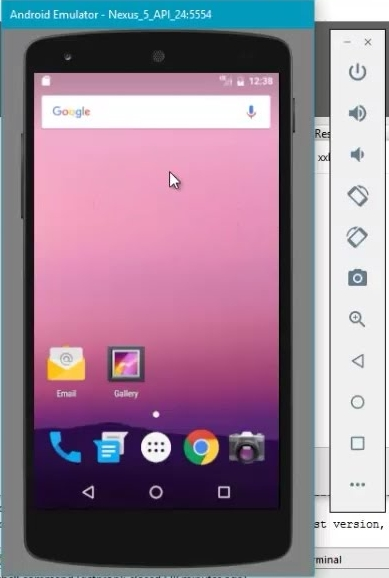
\includegraphics[width=1\linewidth]{figures/avd.jpg}
		\end{itemize}
	\end{minipage}
\end{frame}
\begin{frame}[fragile]{Gradle}
	\begin{minipage}{0.49\textwidth}
		\begin{itemize}
			\item Mavenhez hasonló 
			\item Függőségekkel foglalkozik
			\item Itt tárolja az alkalmazás 
		\end{itemize}
	\end{minipage}
\begin{minipage}{0.49\textwidth}
	\begin{itemize}
		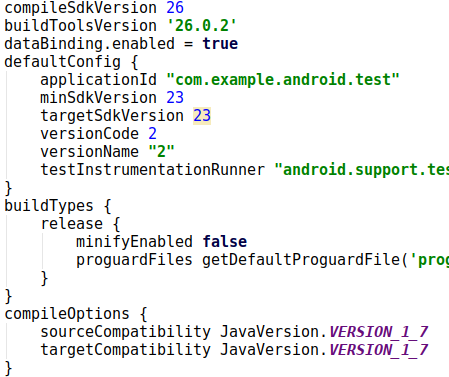
\includegraphics[width=1\linewidth]{figures/gradle.png}
	\end{itemize}
\end{minipage}
\end{frame}
\begin{frame}[fragile]{UI irányelvek}
	\begin{minipage}{0.49\textwidth}
		\begin{itemize}
			\item Kezdőképernyőről nyílik minden 
			\item \textbf{"Lista és részletek"} 
			\item "Körhinta"
			\item Lapok
			\item "Fiók"
		\end{itemize}
	\end{minipage}
	\begin{minipage}{0.49\textwidth}
		\begin{itemize}
			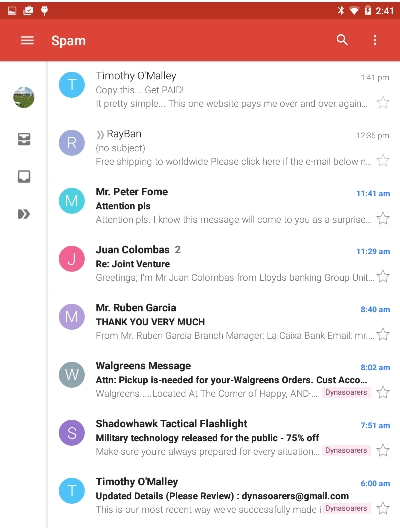
\includegraphics[width=1\linewidth]{figures/listdetails.jpg}
		\end{itemize}
	\end{minipage}
\end{frame}
\begin{frame}[fragile]{UI irányelvek}
	\begin{minipage}{0.34\textwidth}
		\begin{itemize}
			\item Kezdőképernyőről nyílik minden 
			\item "Lista és részletek"
			\item \textbf{"Körhinta"}
			\item Lapok
			\item "Fiók"
		\end{itemize}
	\end{minipage}
	\begin{minipage}{0.65\textwidth}
		\begin{itemize}
			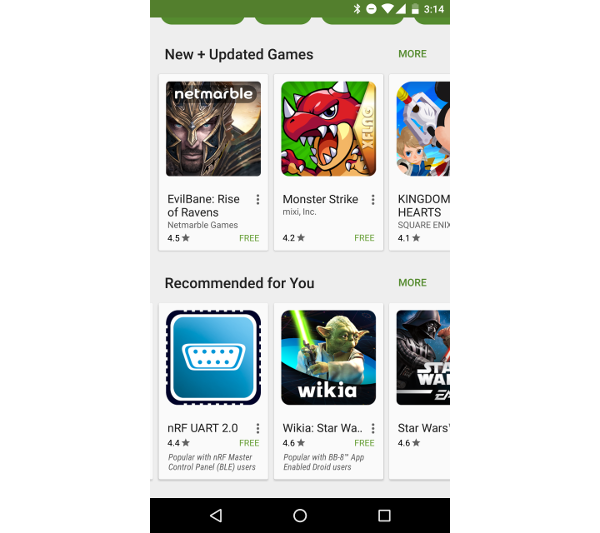
\includegraphics[width=1\linewidth]{figures/googlestorecarousel.png}
		\end{itemize}
	\end{minipage}
\end{frame}
\begin{frame}[fragile]{UI irányelvek}
	\begin{minipage}{0.34\textwidth}
		\begin{itemize}
			\item Kezdőképernyőről nyílik minden 
			\item "Lista és részletek"
			\item "Körhinta"
			\item \textbf{Lapok}
			\item "Fiók"
		\end{itemize}
	\end{minipage}
	\begin{minipage}{0.65\textwidth}
		\begin{itemize}
			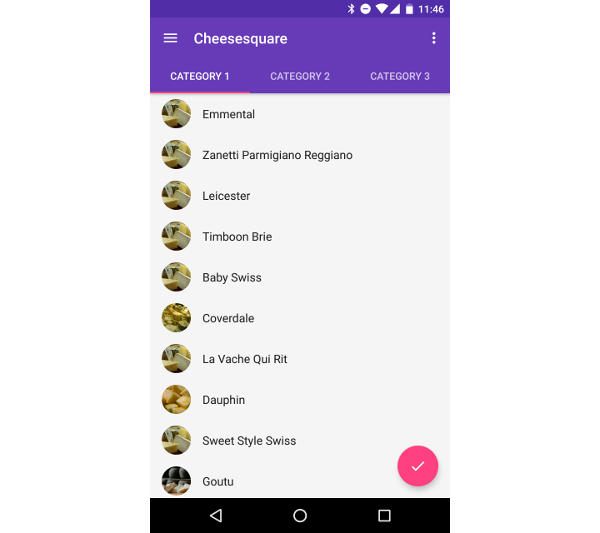
\includegraphics[width=1\linewidth]{figures/viewpagertabs.png}
		\end{itemize}
	\end{minipage}
\end{frame}
\begin{frame}[fragile]{UI irányelvek}
	\begin{minipage}{0.34\textwidth}
		\begin{itemize}
			\item Kezdőképernyőről nyílik minden 
			\item "Lista és részletek"
			\item "Körhinta"
			\item Lapok
			\item \textbf{"Fiók"}
		\end{itemize}
	\end{minipage}
	\begin{minipage}{0.65\textwidth}
		\begin{itemize}
			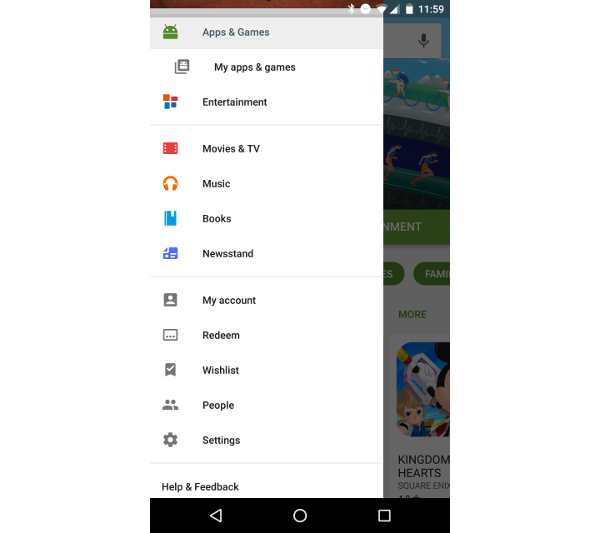
\includegraphics[width=1\linewidth]{figures/drawer.png}
		\end{itemize}
	\end{minipage}
\end{frame}
\begin{frame}[fragile]{Hello World példaprogram}
	\begin{minipage}{1\textwidth}
		\centering
		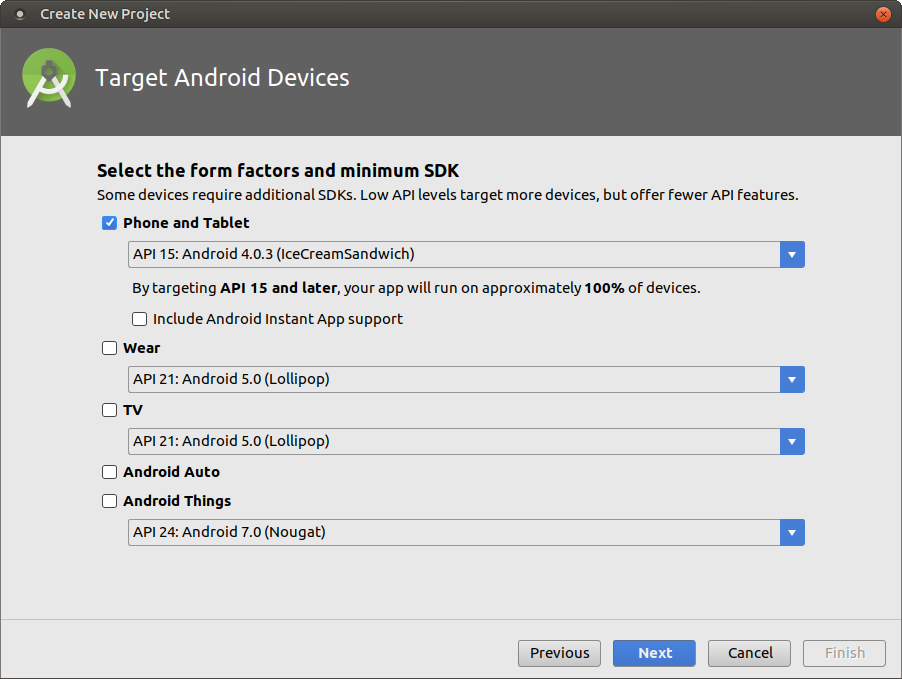
\includegraphics[width=1\linewidth]{figures/hw1.png}
	\end{minipage}
\end{frame}
\begin{frame}[fragile]{Hello World példaprogram}
	\begin{minipage}{1\textwidth}
		\centering
		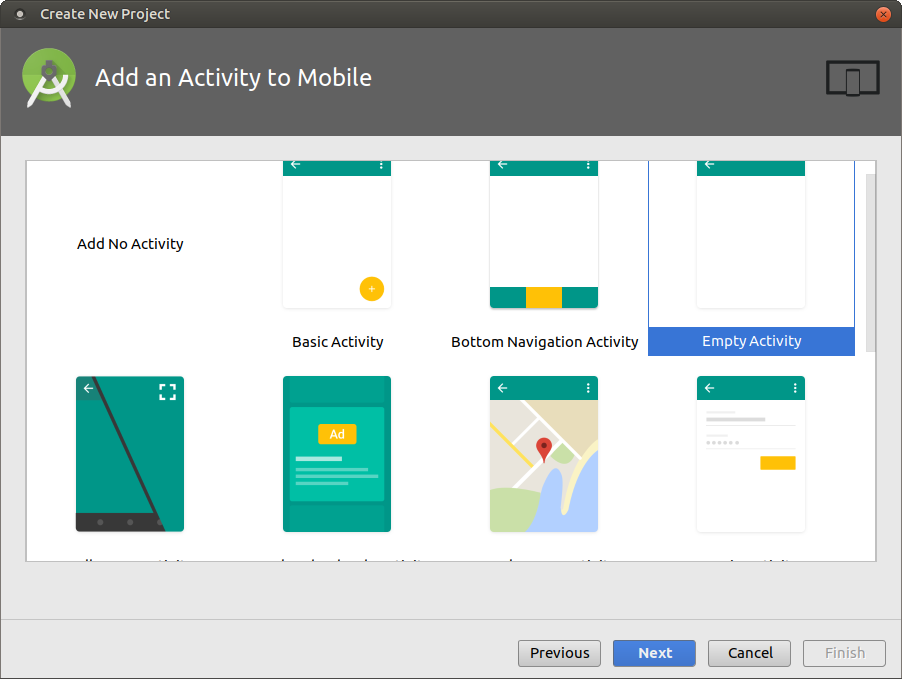
\includegraphics[width=1\linewidth]{figures/hw2.png}
	\end{minipage}
\end{frame}
\begin{frame}[fragile]{Hello World példaprogram}
	\begin{minipage}{1\textwidth}
		\centering
		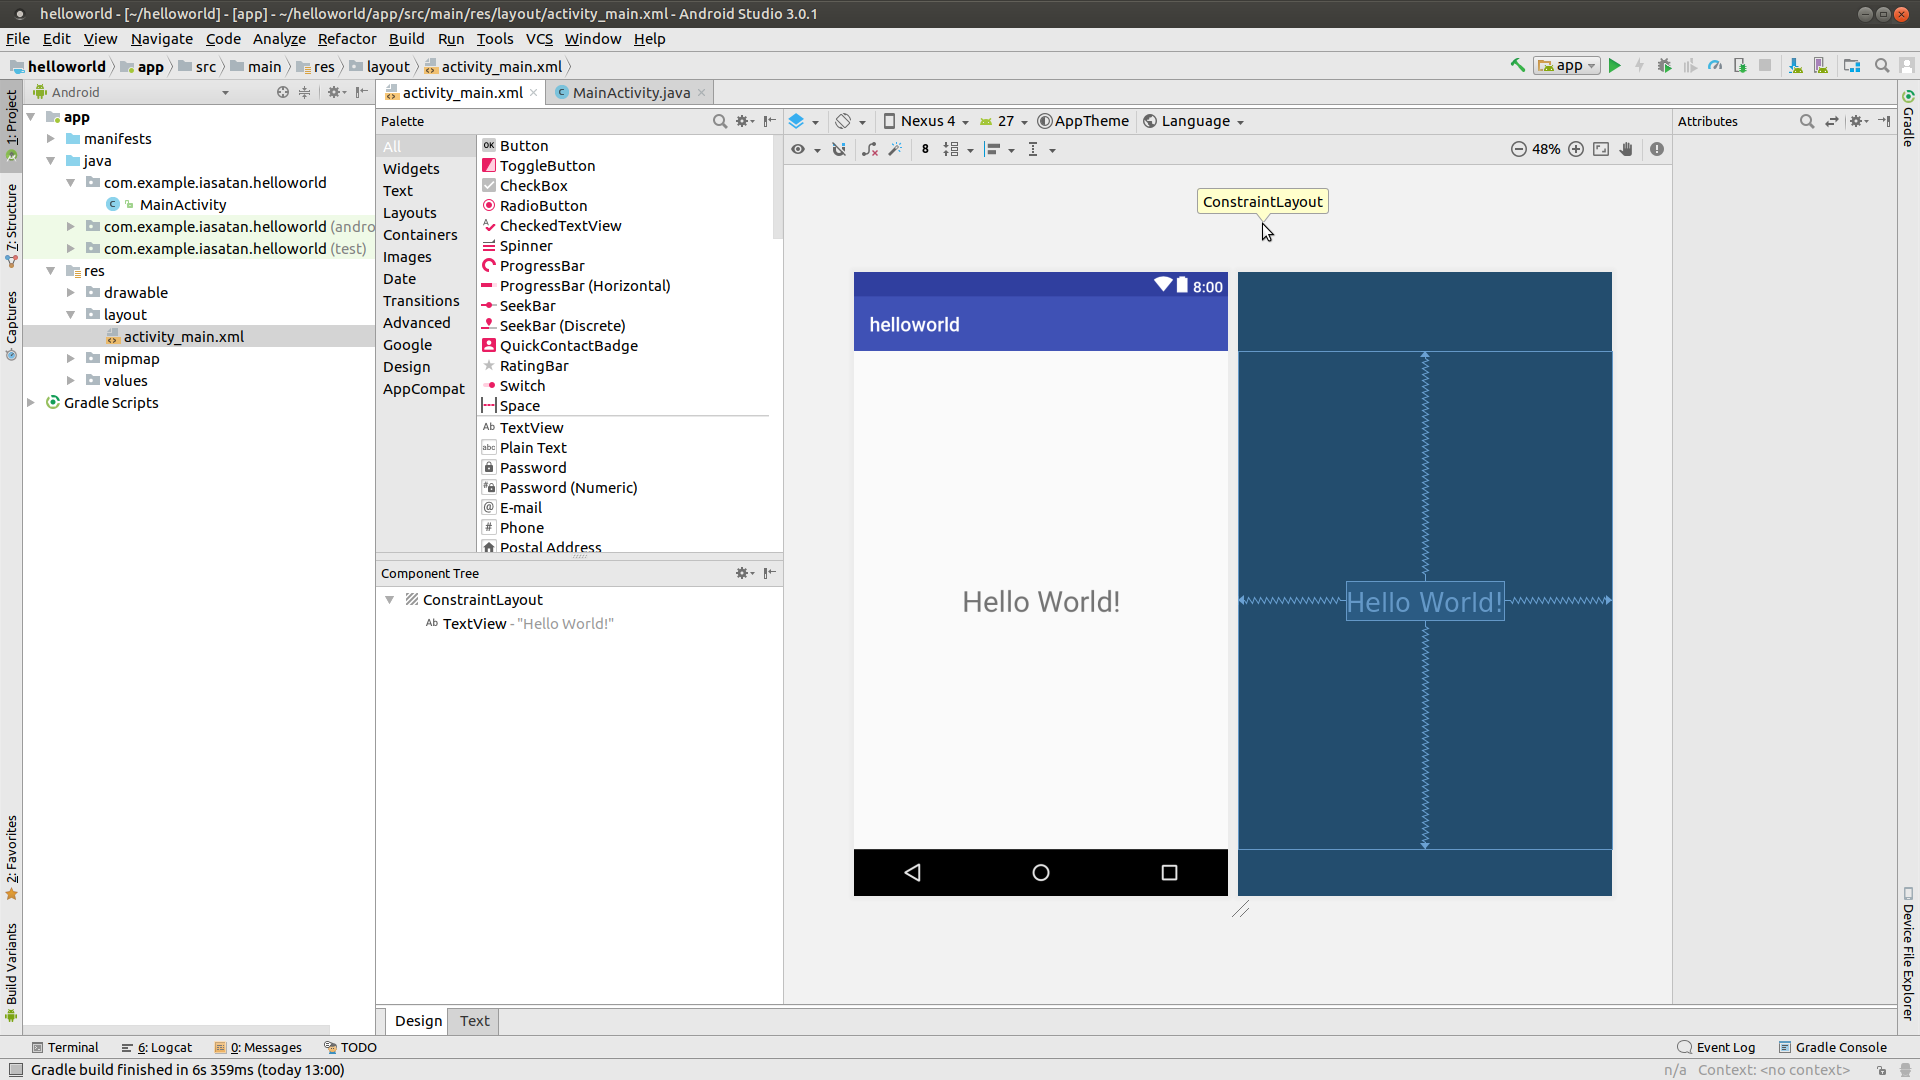
\includegraphics[width=1\linewidth]{figures/h3.png}
	\end{minipage}
\end{frame}
\begin{frame}[fragile]{Saját példaprogram}
	\begin{minipage}{0.49\textheight}
		\begin{itemize}
			\item Belső helymeghatározás
			\item Bluetooth szenzorokon alapul
			\item Tanszéken működik
			\item Lista és részletek 
		\end{itemize}
	\end{minipage}
	\begin{minipage}{0.49\textwidth}
		\centering
		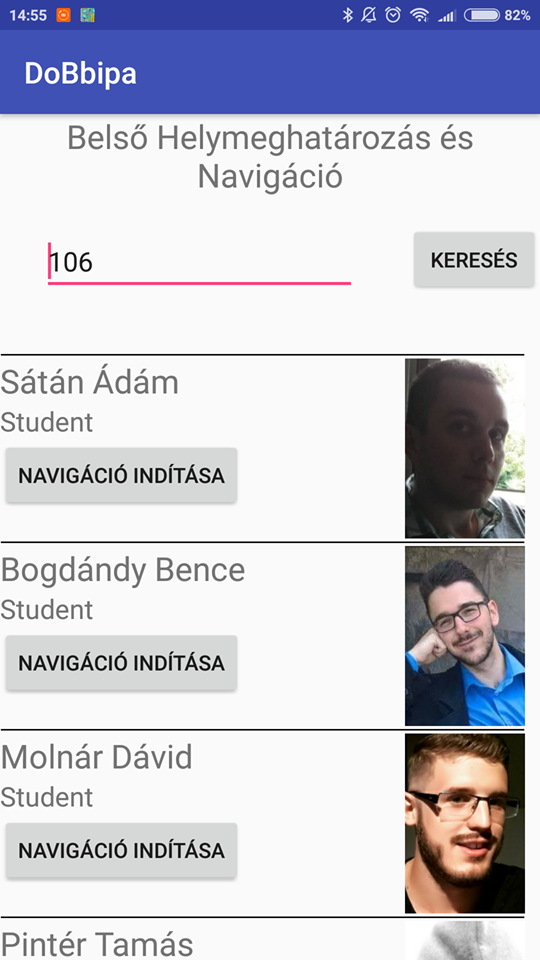
\includegraphics[width=.8\linewidth]{figures/faszok.png}
	\end{minipage}
\end{frame}



\section{Android tesztelés}
\begin{frame}[fragile]{JUnit teszt}
	\begin{minipage}{1\textheight}
		\begin{itemize}
			\item Ugyan az mint Javaban
			\item Metódusok tesztelésére alkalmas
		\end{itemize}
	\end{minipage}
	\begin{minipage}{1\textwidth}
		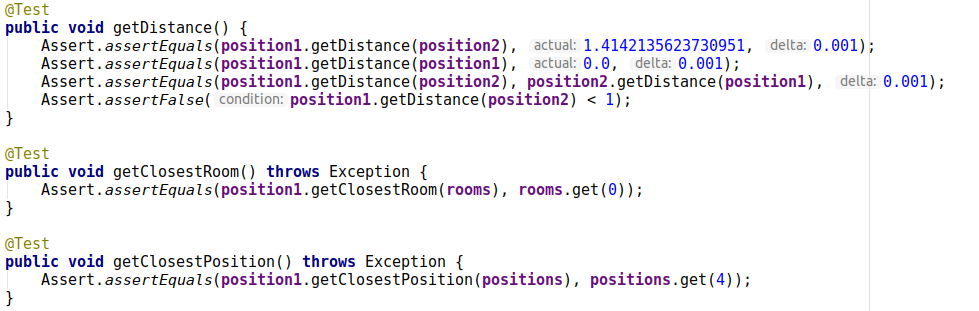
\includegraphics[width=1\linewidth]{figures/junittest.png}
	\end{minipage}
\end{frame}
\begin{frame}[fragile]{Instrumented teszt}
	\begin{minipage}{0.9\textwidth}
		\begin{itemize}
			\item JUnitra épül
			\item Androidon fut a teszt
			\item Android specifikus dolgokat lehet vizsgálni
			\item Különböző Android verziókon, telefonokon és módokon lehet tesztelni 
		\end{itemize}
	\end{minipage}
	\begin{minipage}{1\textwidth}
	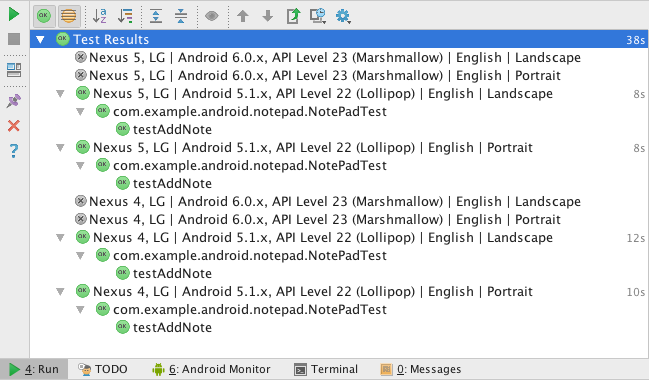
\includegraphics[width=1\linewidth]{figures/ctl-test-results.png}
\end{minipage}
\end{frame}


\section{}
\begin{frame}
\centering
\LARGE Köszönöm a figyelmet!
\end{frame}

\end{document} 